% !TEX root = ../../main.tex
% !TeX spellcheck = de_DE

\chapter{Methodik}
In diesem Kapitel wird die Generierung des Datensatzes beschrieben.
Dabei wird auf die Bildeigenschaften und Besonderheiten der dargestellten Figuren in den Bildern eingegangen.
Außerdem werden die Anforderungen an die Architekturen beschrieben, sowie Ablauf und Kriterien für ein erfolgreiches Training vorgestellt.

\section{Trainingsdaten}
Das Dataset wurde im Rahmen der Studienarbeit generiert und besteht aus 1500 Trainingsbildern.
Die 1500 Bilder teilen sich dabei in jeweils 500 Bilder pro Formklasse (Dreieck, Kreis, Quadrat) auf.
Die genauen Eigenschaften werden in den folgenden Abschnitten beschrieben.

\subsection{Eigener Datensatz}
Zwar gibt es bereits Datensätze mit geometrischen Formen auf Bildern, im Rahmen der Studienarbeit werden jedoch keine vorgefertigten Datensätze verwendet.
Denn die verfügbaren Datensätze entsprechen nicht genau den Anforderungen der Studienarbeit, da die Bilder zum Beispiel farbig, Figuren gedreht oder die Bildgröße nicht mit den Anforderungen übereinstimmt.
Eine Anpassung der Datensätze wäre umständlicher als die Generierung eigener Bilder und würde sowieso einen Vergleich mit anderen GANs, die auf den veröffentlichten Datensätzen basieren, erschweren.
Damit trotzdem eine Vergleichbarkeit zu anderen Arbeiten gewährleistet werden kann, wird die Generierung deterministisch reproduzierbar und dokumentiert sein.

\subsection{Generierung}
Bei den Trainingsdaten handelt es sich um synthetisch generierte Bilder mit geometrischen Figuren. 
Zwar gibt es bereits Datensätze mit ähnlichen Bildern \cite{dataset:2d-geometric-shapes-dataset, dataset:four-shapes}, im Rahmen der Studienarbeit werden jedoch keine vorgefertigten Datensätze verwendet. 
Denn die Generierung eigener Bilder erlaubt eine größere Kontrolle über Eigenschaften der Bilder und Inhalte, als vorgefertigte Sets.
Damit trotzdem eine Vergleichbarkeit zu anderen Arbeiten gewährleistet werden kann, wird die Generierung deterministisch reproduzierbar und dokumentiert sein.

\subsection{Eigenschaften}
Alle Bilder haben eine Größe von 28x28 Pixel und sind Schwarz-Weiß kodiert.
Der Grauwert jedes Pixels wird durch einen Channel angegeben, dessen Werte durch eine Zahl im ganzzahligen Intervall $[0; 255]$ festgelegt ist.
Dabei entspricht die Zahl 0 einem schwarzen Pixel und die Zahl 255 repräsentiert einen weißen Pixel.

Diese Eigenschaften der Bilder entsprechen auch den Bildern des MNIST Datenset \cite{dataset:mnist}, auch wenn sich die Abbildungen unterscheiden.
Durch die relativ kleine Größe lassen sich zum einen Ressourcen beim Training sparen.
Zum anderen erlaubt es die Orientierung der Architektur an diversen Tutorials und Papers zum MNIST Datensatz.
\newline

Auf jedem Bild ist eine geometrische Form abgebildet.
Bei den geometrischen Formen handelt es sich um gleichseitige Dreiecke, Quadrate und Kreise.
Die Formen unterscheiden sich in Größe und Position auf dem Bild.
Andere Transformationen, wie beispielsweise Rotationen, werden nicht angewendet.
Es wird auch kein Rauschen, Weichzeichnen oder Salt and Pepper Noise auf die Bilder angewendet.
\newline

Die Quadrate und gleichseitigen Dreiecke sind zwischen 5 und 16 Pixel groß.
Die Größe bezieht sich dabei auf die Seitenlänge der Seiten.
Die Kreise sind zwischen 5 und 10 Pixel groß.
Hierbei gibt der Wert den Radius des Kreises an.
Die Mindest- und Maximalgrößen sind wichtig, damit die Formen unterscheidbar bleiben.
Bei einer Größe von beispielsweise einem Pixel, wären Kreis, Quadrat und Dreieck identisch.
\newline

Die Formen sind so im Bild positioniert, dass sie Seitenränder touchieren können.
Allerdings ist eine Form immer vollständig im Bild abgebildet und wird vom Bildrand nicht geschnitten.

\newcommand{\trainDataImage}[1]{\subfloat{\fbox{\includegraphics{#1}}}}
\begin{figure}[H]
	\centering
	\trainDataImage{kapitel/3\_methodik/data/circle\_00.png}
	\trainDataImage{kapitel/3\_methodik/data/circle\_01.png}
	\trainDataImage{kapitel/3\_methodik/data/circle\_02.png}\par 
	
	\trainDataImage{kapitel/3\_methodik/data/rectangle\_00.png}
	\trainDataImage{kapitel/3\_methodik/data/rectangle\_01.png}
	\trainDataImage{kapitel/3\_methodik/data/rectangle\_02.png}\par 
	
	\trainDataImage{kapitel/3\_methodik/data/triangle\_00.png}
	\trainDataImage{kapitel/3\_methodik/data/triangle\_01.png}
	\trainDataImage{kapitel/3\_methodik/data/triangle\_02.png}\par 
	
	\caption{Auswahl an zufällig generierten Trainingsbilder}
\end{figure}

\section{Bewertungskriterien}
Damit ein Vergleich zwischen den Architekturen gezogen werden kann, müssen Kriterien für ein erfolgreich trainiertes GAN klar definiert werden.
Als Erfolgskriterien zählen in diesem Fall die Varietät der generierten Bilder und die Korrektheit der generierten Figuren.
Beide Kriterien werden im Folgenden noch einmal genauer erläutert.

\subsection{Varietät}
Die Varietät bezieht zum einen auf die Ähnlichkeit zwischen Trainingsbildern und den generierten Bildern der GANs.
Die Ähnlichkeit zwischen diesen beiden Bildersets beschreibt, wie gut das GAN 'etwas neues schaffen' kann, oder ob es nur Trainingsbilder dupliziert.
Sollte die Ähnlichkeit sehr gering sein, werden viele 'neue' Bilder generiert, was sehr positiv zu bewerten ist.
\newline

Zudem bezieht sich die Varietät auf die generierten Bilder untereinander.
Sie sollten auch möglichst verschieden sein, was oftmals nicht der Fall ist.
Das Phänomen ist als 'mode-collapse' bekannt. \todo{ist mode-collapse im stand der technik?}
% https://scikit-image.org/docs/0.12.x/api/skimage.measure.html#skimage.measure.compare_ssim

\subsection{Korrektheit}
Neben der Varietät besitzt auch die Korrektheit eine hohe Bedeutung für die Bewertung der GANs.
Dafür muss sichergestellt werden, dass die richtige Figur zum zugehörigen Label generiert wurde und erkennbar ist.
Die Figuren müssen außerdem den gleichen Kriterien wie die Trainingsdaten genügen, das heißt, die Figuren sollten zum Beispiel vollständig innerhalb des Bildes abgebildet sein.
\newline

Ein weiterer wichtiger Aspekt der Bilder ist das Verhalten im Hintergrund der Figur.
So sollten im Hintergrund möglichst keine anderen Figuren oder Pixelfragmente erzeugt werden.

\subsection{Bestimmung}
Sowohl Varietät als auch Korrektheit können mit der \acrlong{FID} \cite{frechet-inception-distance} gemessen werden.
Dadurch wird ein objektiver Vergleich zwischen den Architekturen gewährleistet.
\newline

Zusätzlich erfolgt eine manuelle Überprüfung der Endresultate.
Eine manuelle Überprüfung ist zwar subjektiv, verhindert allerdings, dass gute Ergebnisse aufgrund von Ungenauigkeiten der \acrshort{FID} übersehen werden.

\section{Training}
Im Trainingsprozess werden verschiedene Architekturen mit unterschiedlichen Hyperparametern getestet.
Die ausgewählten Architekturen orientieren sich an bereits existierender Forschung und Tutorials (siehe \cref{chapter:related-work}).
Insbesondere aufgrund der Label-Abhängigkeit (im Rahmen der Studienarbeit entsteht ein Conditional-GAN) werden jedoch Anpassungen erfolgen.


\subsection{Auswahl zu optimierender Hyperparameter}
Die eigentliche Suche und Optimierung der Hyperparameter läuft automatisch ab.
Allerdings können aufgrund von endlichen Ressourcen nicht alle Hyperparameter-Kombinationen getestet werden.
Darum muss sich zuvor manuell auf die vielversprechenden Hyperparameter beschränkt werden.
\newline

Natürlich existieren so genannte Auto-Machine-Learning Systeme, welche ohne Vorauswahl vollautomatisch Architektur und Hyperparameter optimieren können. 
Jedoch erreichen diese nicht immer die gleiche Leistung wie manuell optimierte Modelle.
So zeigt eine Versuch aus dem Jahre 2021, dass die Bibliothek AutoKeras \cite{auto-keras} auch nach 24 Stunden Optimierungs-Zeit nicht die Genauigkeit eines von Hand eingestellten Modells erreicht \cite[S. 2036]{dl-framework-evaluation}.
\newline

Die auszuwählenden Hyperparameter sollen dabei zum einen eine vergleichsweise hohe Auswirkung auf den Trainingserfolg haben.
Zum anderen sollen sie sehr allgemein sein, um sie gleichermaßen auf die verschiedenen Architekturen anwenden zu können.
Das garantiert eine bessere Vergleichbarkeit zwischen den Architekturen.
\newline

Die Hyperparameter \textit{Batch-Size}, \textit{Learning-Rate Generator}, \textit{Learning-Rate Discriminator}, \textit{Dropout} und \textit{Smoothness} entsprechen diesen Voraussetzungen.

\subsubsection{Learning-Rate}
Die Learning-Rate entspricht dem Faktor \(\alpha\), welcher die Intensität des Gradientenabstiegs bestimmt:  

\[\theta_{}  =  \theta_{}  - \alpha   \nabla_{ \theta }  J( \theta )  \]

\todo[]{mit quellen backen}
Bei zu großem \(\alpha\) kann der Trainings-Fehler anfangen zu oszillieren oder sogar größer werden.
Bei zu kleinem \(\alpha\) konvergiert der Fehler zu langsam oder bleibt in einem lokalen Minimum stehen. 
Es ist anzumerken, dass die oben gezeigt Formel dem einfachen Gradientenabstieg entspricht.
Normalerweise werden fortgeschrittenere Algorithmen angewendet, welche jedoch weiterhin auf dem Gradientenabstieg basieren.
So können weitere Parameter, wie das \textit{Momentum} die Abstiegsweite beeinflussen.
\newline

Daraus lässt sich schließen, dass im Fall von Adam die Lernrate vor allem am Anfang des Trainings bedeutend ist.
Nichtsdestotrotz hat die Learning-Rate auch einen großen Einfluss auf das Ergebnis und gilt allgemein als einer der wichtigsten Hyperparameter \cite[S. 447]{learning-rate-most-important}. 
\newline

Die Signifikanz sticht vor allem bei einem GAN heraus, da dort die Learning-Rate für Generator und Discriminator unabhängig gesetzt werden kann.
Unterschiedliche Werte können dazu führen, dass eines der Modelle seinen Gegenspieler völlig dominiert.
Auf der anderen Seite, können mittels unterschiedlichen Parameter etwaige Schwächen eines Modells ausgeglichen werden.
Es ist also dementsprechend wichtig, mehrere Kombinationen von verschiedenen Lernraten zu untersuchen.
\newline

Vor der Studienarbeit gesammelte Erfahrungen haben gezeigt, das eine Lernrate im Bereich von \(2e-3\) bis \(2e-5\) für die geplanten Modelle gut funktionieren.
Außerdem wurden diese Werte häufig in Adam-bezogene Tutorials referenziert \cite{adam-tutorial}.
Für die Hyperparamter-Suche werden deshalb für Generator und Discriminator die gleichen vier Lernraten festgelegt:

\begin{center} \(2e-3\), \(2e-4\), \(3e-4\) und \(2e-5\). \end{center}

Einerseits ist so ein symmetrischen Training mit guten Erfahrungswerten möglich.
Anderseits sollen durch die gewählten Werte asymmetrische Trainings mit drei verschiedenen Abständen untersucht werden:
\begin{itemize}
	\item ein sehr großer Abstand von zwei Dezimalstellen
	\item ein großer Abstand von einer Dezimalstelle
	\item ein kleiner Abstand von \(1e-4\)
\end{itemize}	

\subsubsection{Batch-Size}

Deshalb muss ein Kompromiss gefunden werden.
\newline

\(32\) wird in Papers oder Tutorials häufig als ein guter Standartwert angegeben \cite{default-batch-size}.
Jedoch sollen in der Studienarbeit mehre Architekturen mit einer großen Anzahl an Hyperparametern untersucht werden.
Gleichzeit sind die verfügbaren Ressourcen begrenzt, weshalb eine größere Batch-Size eine schnellere Hyperparameter-Suchen ermöglichen würde.
Aus diesem Grund wird für die erste Untersuchung neben der Batch-Size von \(32\) auch \(64\) getestet.

\todo[]{begründung und welche werte und warum} 
\subsubsection{Dropout}
Beim Dropout wird ein gewisser Teil der Neuronen einer Schicht deaktiviert.
Das passiert jedoch nur während dem Training und führt dazu, -> gegen overfitting
https://machinelearningmastery.com/dropout-for-regularizing-deep-neural-networks/



\todo[]{begründung und welche werte und warum} 
\subsubsection{Smoothness}
Die Smoothness entstammt einer Idee von Ian Goodfellow \cite{ian-goodfellow-onesided-label-smoothing}.
\newline

Alle festgelegten Hyperparameter finden sich in der folgenden Tabelle \ref{table:hyperparameter} nochmals zusammengefasst.
Dementsprechend müssen insgesamt 72 Kombinationen pro Architektur getestet werden. \todo{72 nicht korrekt}
Es ist jedoch anzumerken, dass spätere Anpassungen an der Hyperparameter-Auswahl möglich sind.
Vor allem falls es sich heraus stellt, dass einige Werte in keiner Kombination gute Ergebnisse erzeugen.

\todo{tabelle nicht korrekt}
\begin{table}[H]
	\centering
	\label{table:hyperparameter}
	\begin{tabular}{l l}
		Name                        & Werte            \\ \hline
		Batch Size                  & 16, 32           \\
		Dropout                     & 0.3, 0.4         \\
		Smoothness                  & 0, 0.1           \\
		Learning-Rate Discriminator & 2e-3, 2e-4, 3e-4 \\
		Learning-Rate Generator     & 2e-3, 2e-4, 3e-4
	\end{tabular}
	\caption{Allgemeine Hyperparameter Auswahl}
\end{table}

\subsection{Trainingsablauf}
Vor der Implementierung und Analyse der verschiedenen Architekturen werden zunächst die Trainingsdaten generiert.
Danach erfolgt die Implementierung einer neuen Architektur und Festlegung der Hyperparameter.
Schließlich wird das Training durchgeführt.
Beim Training wird automatisch eine Grid Search durchgeführt und Logs für diverse Werte berechnet.
Die Logs können im Anschluss mithilfe von Tensorboard visualisiert werden.

\subsection{Logs}
Während des Trainings wird eine Reihe von Logs zur Analyse erzeugt.
Alle Metriken in den Logs werden dabei auf Testdaten angewendet, um ein Overfitting erkennen zu können.
Die genauen Werte und die mit dem Logging verknüpften Intentionen werden im Folgenden erläutert.
\newline

Während dem Training werden mehrere Werte geloggt.
Ein Wert ist dabei der Loss, sowohl für den Generator, als auch für den Discriminator.
Der Loss wird für jede Epoche geloggt und ist vor allem zur Analyse des Trainingsprozesses interessant.
So können schlechte Trainingsdurchläufe schon früher abgebrochen werden und zugehörige Architekturen verbessert werden.
\newline

Für die Auswertung sind vor allem die generierten Bilder und der \acrshort{FID}-Index relevant.
Die Bilder werden nach jeder Epoche mit einer immer identischen Latent-Dim erzeugt.
Dadurch ist eine bessere Vergleichbarkeit gewährleistet.
Tensorboard erlaubt dann eine Ansicht mit Zeitachse, um den Lernprozess über die verschiedenen Epochen beobachten zu können.
\newline

Der \acrshort{FID}-Index ist sehr aufwändig zu berechnen.
Deshalb wird er erst am Ende mit den finalen Bildern erzeugt.
Bei einem Overfitting könnten so theoretisch schlechtere Ergebnisse für ein Modell entstehen.
Durch eine zusätzliche manuelle Analyse über die einzelnen Epochen und der vergleichsweise geringen Epochenanzahl ist das Risiko einer potentiellen Verfälschung der Ergebnisse jedoch sehr gering.
\newline

Die gesammelten Daten sind alle nach Architektur und Hyperparameterkombination unterteilt abgespeichert.
Die Unterteilung erlaubt die Auswahl einer möglichst optimalen Kombination aus beidem.

\section{Verfahren zur Hyperparametersuche}
Die Suche nach optimalen Hyperparametern ist sehr komplex, weswegen spezielle Suchverfahren entwickelt wurden.
Die Manuelle Suche, Grid Search, Random Search und der Genetic Algorithm werden deshalb auf ihre Anwendbarkeit in der Studienarbeit verglichen und ein passendes Verfahren ausgesucht.


\subsection{Kriterien}
In diesem Abschnitt werden Kriterien für die Auswahl eines geeigneten Hyperparameter Suchverfahrens ausgewählt.

\subsubsection{Automatisierbarkeit}
Ziel ist es, pro Nacht eine Architektur zu trainieren.
Deswegen ist es wichtig, dass das Verfahren vollkommen automatisiert ablaufen kann.

\subsubsection{Ressourcenbedarf}
Das Verfahren darf in keinem Fall während oder nach einer Trainingsiteration so viel zusätzlichen Speicher belegen, dass das Training oder das Speichern der Logs fehlschlägt.
Der verfügbare Arbeits- und Grafikkartenspeicher nicht ausreichend, um Trainingsdurchläufe stark zu parallelisieren.

\subsubsection{Laufzeit}
Die Laufzeit der Hyperparametersuche ist von entscheidender Bedeutung.
Denn die verwendete Hardware ist nicht ausreichend, um jegliche Kombinationen von Hyperparametern in einer vernünftigen Zeit zu testen.
Als zeitliche Begrenzung dient dabei die Ausführung von allerhöchstens 8h.
\newline

Jedoch ist zu beachten, dass auch der Trainingsprozess als solcher viel Zeit in Anspruch nimmt.
Der reine Trainingsaufwand erlaubt mit der verwendeten Hardware in den 8h maximal 75 sequentielle Trainingsdurchläufe (je nach Architektur kann der genaue Wert abweichen).
Folglich sollte das Verfahren innerhalb von 75 Durchläufen zu einem Ergebnis kommen.

\subsubsection{Effektivität}
Das Verfahren soll in jedem Fall eine gute Kombination im zeitlichen Rahmen finden.
Das ist insofern wichtig, als dass ansonsten kein Vergleich zu anderen Architekturen erfolgen kann.
Aufgrund der geringen Ressourcen (Zeit und Rechenleistung) besteht zwar kein Anspruch auf Optimalität, jedoch sollte es zumindest ein gutes Ergebnis liefern.

\subsubsection{Implementierungsaufwand}
Der zusätzlich verursachte Implementierungsaufwand ist nicht so wichtig wie die anderen Kriterien.
Er kann aber als Ausschlusskriterium bei ähnlich guten Verfahren dienen.
Der Implementierungsaufwand wird durch Dokumentation, Tutorials, Libraries, oder eine Einbindung in Tensorflow/-board verringert.

Bei der Verwendung von Libraries ist essentiell, dass sie eigene Trainingsfunktionen und den spezielleren Trainingsablauf von GANs unterstützen.
Zusätzlich müssen sie in jedem Fall mit Tensorflow oder Keras kompatibel sein.

\subsection{Vergleich}
In diesem Abschnitt werden die vorgestellten Verfahren miteinander auf Basis der Kriterien verglichen.

\subsubsection{Manuelle Suche}
Die manuelle Suche ist aufgrund der ständigen verpflichtenden Neuevaluierungen der Traingsergebnisse als einziges Verfahren \todo{reicht es nur Automatisierbarkeit nur in der manuellen suche anzusprechen?} nicht automatisierbar.
Zudem erhöhen die Evaluierungen den Zeitaufwand zusätzlich, da jedes mal eine fundierte Entscheidung getroffen werden muss.
Insgesamt erhöht sich so die Laufzeit im Vergleich zu automatisierten Verfahren sehr stark.
\newline

Alle anderen Kriterien werden hingegen optimal erfüllt.
Denn für die Einführung einer manuellen Suche müssen keinerlei Anpassungen am Trainingsprozess oder Code vorgenommen werden.

\subsubsection{Grid Search}
Die Laufzeit der Grid Search hängt stark von der Anzahl der Hyperparameter ab.
Das liegt an der Durchführung eines Trainings für jede mögliche Kombination aus den Hyperparametern.
Im Rahmen der Studienarbeit werden jedoch nur wenige bestimmte Hyperparameter getestet, wodurch eine ausreichend schnelle Laufzeit gegeben ist.
Zwar könnte das Verfahren insgesamt durch Parallelisierung noch beschleunigt werden, das würde allerdings die Hardwarekapazitäten übersteigen.
Bei einem sequentiellen Ablauf stellt die Ressourcennutzung keine Probleme dar.
\newline

Die Effektivität des Verfahrens ist auch gegeben, solange eine geeignete Kombination aus den Hyperparameterwerten gebildet werden kann.
Sollte keine gute Kombination im Suchraum existieren, scheitert das Verfahren.
Dementsprechend wichtig ist die Wahl der Werte.
Die Effektivität kann allerdings mit Verfahrensanpassungen sogar erhöht werden.
Zwar findet die Grid Search in keiner intelligenten Weise die optimalen Hyperparameter, aber durch kurze Trainings- und Validierungsintervalle können schlecht trainierende Kombinationen schnell aussortiert werden.
Das erlaubt ein viel größeren Suchraum und somit auch eine effektivere Suche.
\newline

Die Implementierung in das Projekt ist sehr einfach, da eine Grid Search native von Tensorflow unterstützt wird.
Durch eine Iteration über das Kreuzprodukts aller Hyperparameterwerte lässt sich dann die Suche umsetzen.
Durch den simplen Neustart des Trainings werden auch automatisch eigene Trainingsfunktionen oder -abläufe unterstützt.

\subsubsection{Random Search}
Die Random Search ist der Grid Search sowohl im Verhalten als auch in der Bewertung sehr ähnlich.
Auch bei der Random Search sind Ressourcenbedarf und Laufzeit vertretbar, solange das Verfahren nicht parallelisiert wird und nicht zu viele zufällige Werte für die Hyperparameter ausgewählt werden.
\newline

Statt der Wahl der Werte beeinflusst bei diesem Verfahren die Wahl der Intervalle die Effektivität.
Diese müssen so klein gewählt werden, dass bei der Anzahl an generierten Werten eine Chance besteht, optimale Werte zu finden.
Das bedeutet einem Intervall von 100 möglichen Werten sollte nicht nur 1 Zufallswert gegenüberstehen. \todo{in Stand der Technik?}
\newline

Der Implementierungsaufwand ist etwas größer als bei der Grid Search.
Zwar gibt es das Package KerasTuner \cite{omalley2019kerastuner}.
Der KerasTuner hat allerdings keine Dokumentation zu eigenen Trainingsabläufen/-funktionen, die beim GAN zum Einsatz kommen.
Allerdings können die Werte auch ohne den KerasTuner erzeugt und dann wie bei der Grid Search verwendet werden.
Dann fehlt jedoch eine Funktion, die eine \textit{Automatic Relevance Determination} über die Werte ausführt.

\subsubsection{Genetic Algorithm}
Die Laufzeit des Genetic Algorithms ist bei wenigen Hyperparametern vergleichsweise hoch.
Dafür nimmt die Laufzeit bei mehr Hyperparametern in nur geringem Maß zu.
Jedoch wird für die Studienarbeit eine stark begrenzende Vorauswahl an Hyperparametern getroffen. \todo{Wo begründet?}
Dadurch ist die Laufzeit des Verfahrens vergleichsweise hoch.

Durch eine mangelnde Parallelisierung müssen auch alle Modelle in einem Evolutionsschritt sequentiell trainiert werden.
Da es sich dabei beispielsweise um 50 (Standardwert für Tensorflow Optimierung) parallele Modelle handelt, ist steigert das die Laufzeit sehr stark.
\newline

Die Effektivität des Verfahrens ist gegeben, wenn es komplett durchlaufen kann.
Das ist aufgrund der hohen Laufzeit allerdings fraglich.
Sobald das Verfahren früher abgebrochen wird, muss keine Effektivität mehr vorhanden sein.
Insbesondere unter der Annahme, dass sich die Hyperparameter stetig anpassen und optimieren \todo{und das netz nicht übertrainiert wurde}, sollte sogar ein deutlich schlechteres Ergebnis geliefert werden, als am Ende herauskommt.
\newline

Für die Implementierung stellt Tensorflow eine Optimierungsfunktion bereit.
Jedoch unterstützt die Funktion keine eigenen Trainingsabläufe, oder es ist nicht dokumentiert.
Aufgrund der fehlenden Informationslage ist der tatsächliche Aufwand nur schwer einschätzbar. %TODO \todo{nochmal recherchieren?}
Er sollte jedoch deutlich höher liegen, als bei den anderen beiden Verfahren.

\subsection{Bewertung}

\begin{table}[H]
	\centering
	\begin{tabular}{l|c|c|c}
		                        & Grid Search & Random Search & Genetic Algorithm \\
		Automatisierbarkeit     &      +      &       +       &         +         \\
		Ressourcenbedarf        &      +      &       +       &         o         \\
		Laufzeit                &      +      &       +       &         -         \\
		Effektivität            &      o      &       o       &        ++         \\
		Implementierungsaufwand &      +      &       o       &         -
	\end{tabular}
	\caption{Bewertung der Hyperparameterverfahren}
\end{table}


Die manuelle Suche ist viel zu aufwändig und für moderne Suchen nicht mehr zeitgemäß, da eine Automatisierung fehlt.
Für eine derart intensive Suche fehlen die Ressourcen und der dabei entstehende Aufwand wiegt auch nicht den Nutzen auf.
\newline

Der Genetic Algorithm ist zwar an sich ein sehr guter Algorithmus.
Allerdings ist das Projekt zu klein und die Hardware zu beschränkt, um ihn richtig ausnutzen zu können.
Bei größeren Projekten und vor allem bei weniger ressourcenaufwändigen Trainingsdurchläufen als Bildgenerierungen mithilfe von GANs ist er allerdings definitiv vorzuziehen.
Das liegt vor allem an der allgemeinen Suchart, bei der jegliche Kombination und diverse Hyperparameter in Betracht gezogen werden können.
\newline

Sowohl die Grid Search als auch die Random Search sind geeignete Verfahren im Rahmen dieser Arbeit.
Sie sind sich so ähnlich, dass auch ihre Vorteile und Nachteile sich nicht stark unterscheiden.
Die Verfahren sind vor allem aufgrund ihrer geringen Laufzeit bei wenigen Hyperparametern und der trotzdem guten Effektivität gewählt.

Ausschlaggebend unterscheiden sich die Verfahren nur in der Implementierung.
Hierbei ist die Grid Search der Random Search etwas überlegen und wird deshalb implementiert.

\section{Architekturen}
Es werden zwei verschiedene Architekturen untersucht und miteinander verglichen.
Das Dense GAN soll auf dem Dense Layer basieren, wohingegen das DC GAN sich auf das Convolutional Layer stützt.
Ziel ist, die beiden Techniken zu vergleichen und den Einfluss verschiedener Hyperparameter zu evaluieren.

\subsection{Gemeinsamkeiten}
Um beide Architekturen in die Trainingsumgebung einbinden zu können, müssen sie die gleichen Ein- und Ausgaben besitzen.
Das ermöglicht jedoch nicht nur eine einfachere Implementierung, sondern macht ebenfalls die Evaluierung einfacher.
Die Anforderungen an die Ein- und Ausgabe sind wie folgt definiert.
\newline

Der Discriminator erhält als Eingabe ein Bild als Array und zusätzlich ein Label als Skalar.
Die Bild-Input hat den Formfaktor \textit{[28,28]}, wobei jeder Pixel als Graustufe zwischen \textit{0} und \textit{255} übergeben wird.
Das Label wird per \textit{Ordinal Encoding} repräsentiert.
Dabei werden den einzelnen Klassen ein Integer zugewiesen, was in diesem Fall zu einem Skalar zwischen 0 und 2 führt.
Es wurde sich für dieses Codierung entschieden, da sie verglichen zur \textit{One-Hot Encoding}, bei der die Labels von einem Vektor dargestellt werden, einfacher zu implementieren ist \cite{label_encoding}.
Die Ausgabe des Discriminators ist eine Zahl zwischen 1 und -1, welche die vorhergesagte Echtheit angibt.
Eine 1 bedeutet, dass das gegeben Bild real ist, eine -1 wiederum, dass es vom Generator stammt.
\newline

Der Generator erhält als Eingabe einen 100 Stellen langes Array mit Zufallszahlen (Latent-Dimension) und den gleichen Label-Skalar, den auch der Discriminator erhält.
Die Zufallszahl wird dabei als Vektor übergeben.
Die Ausgabe des Generators entspricht dem bereits beschrieben Bild.
Logischerweise muss dieser Output mit der Bild-Eingabe des Discriminators übereinstimmen, also einer Matrix in der Form \textit{[28,28]}.

\subsection{Dense GAN}
\label{section:dense-gan}
Das Dense GAN ist an einem Tutorial für das MNIST Datenset inspiriert.\todo{quelle}
Diese Architektur zeichnet vor allem aus, das zur Verarbeitung ausschließlich Dense-Layer zum Einsatz kommen.
Die Architektur wurde zu großen Teilen aus der Vorlage übernommen.
Die größte Abweichung liegt in dem hinzugefügten Label-Input, da im Tutorial nur ein GAN ohne Konditionalisierung beschrieben wurde.

\subsubsection{Discriminator}
In der Abbildung \ref{architecture:densegan-dis-input} sind die beiden Eingabe Schichten des Disciminators und ihre Vereinigung zu erkennen.
Beide Eingaben werden vor den Verarbeitung, also den Dense Schichten, miteinander verbunden.
Das steht zum starken Kontrast des DC-GAN Discriminators, da dort erst beide Inputs verarbeitet und anschließend multipliziert werden.
Es handelt sich dabei schlicht um zwei verschiedene Ansätze, welche deutlicher werden, sobald der Discriminator des DC-GAN beschrieben wird.

\begin{figure}[H]
	\centering
	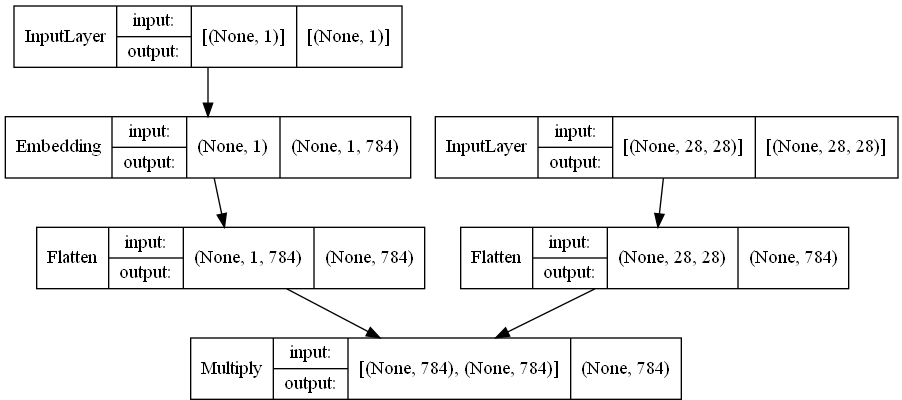
\includegraphics[height=0.3\textheight]{kapitel/5_ergebnisse/architectures/densegan_discriminator/inputs.png}
	\caption{Inputs des Dense-GAN-Discriminators}
	\label{architecture:densegan-dis-input}
\end{figure}

Ein wichtiger Schritt ist das Angleichen des Bild und Labels.
Die später folgenden DenseLayer sollen mit Vektoren arbeiten, weshalb beide Eingaben zu einem gleich großen Vektor umgeformt werden.
Das Bild wird durch eine Flatten Schicht von Matrix in eine Vektor Form gebracht. 
Dabei werden die einzelnen Neuronen einfach in eine Reihe verschoben, ohne irgendwelche Anpassungen an den Werten vorzunehmen.
Somit erklärt sich auch die Vektorlänge: \begin{equation}
	28 * 28 = 784.
\end{equation}
Um das Label auf die gewünschte Länge zu bringen, wird der Skalar \textit{embeddet}.
Dadurch wird jeder Klasse einen eigener Vektor mit der Länge \textit{784} per Gewichte zugewiesen.
Dieser spezieller Vektor repräsentiert dementsprechend eine ganz bestimmtes Label, welche anschließend mit dem Bild-Vektor multipliziert wird.
\newline

In der Abbildung \ref{architecture:densegan-dis-dense} ist der zweite Zeil des Diskriminators zu erkennen.
Nach der Multiplikation werden die mit dem Label kombinierten Bilddaten mittels vollverbunden Schichten verarbeitet.
Dabei besteht jeder Verabeitungsschritt aus einem DenseLayer, gefolgt von der LeakyReLU Aktivierungsfunktion.
Drei dieser Schritte existieren, wobei sich bezüglich der einzelnen Output-Größen stark an das Tutorial orientiert wurde.
Als erstes wird der Vektor auf \textit{128} verkleinert.
Anschließend wird die Länge zwei mal verdoppelt, sodass am Ende ein Vektor mit der Größe von \textit{512} ausgegeben wird.

\begin{figure}[H]
	\centering
	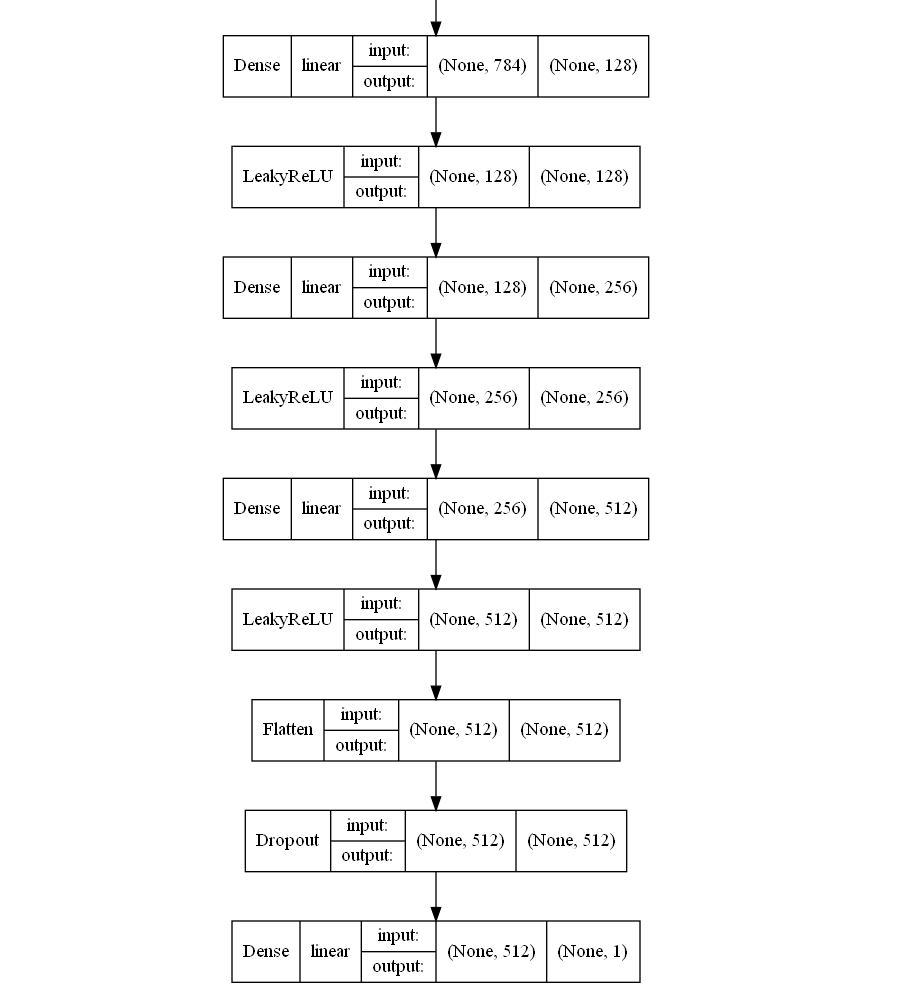
\includegraphics[width=0.6\textheight]{kapitel/5_ergebnisse/architectures/densegan_discriminator/dense.png}
	\caption{Verabeitungs Schichten des Dense-GAN-Discriminators}
	\label{architecture:densegan-dis-dense}
\end{figure}

Nach den Verabeitungsschichten wird zunächst noch der Dropout angewendet.
Die Funktion des Droupouts wurde bereits im Kapitel der Hyperparameter beschrieben.
Anschließend müssen die Neuronen per Dense Schicht komprimiert werden.
Dadurch wird ein einziges Output-Neuron erreicht, welches die Vorhersage des Discriminators darstellt.

\subsubsection{Generator}
Wie bereits beschrieben, besitzt der Generator zwei Eingaben: das Label und den Latent-Vektor.
In der Abbildung \ref{architecture:densegan-gen-input} sind diese dargestellt.
Auch der Generator arbeitet innerhalb seiner DenseLayer mit einem Vektor.
Dementsprechend muss der Latent-Input nicht weiter vorverarbeitet werden und wird direkt in das MultiplyLayer gereicht
Lediglich das Label wird ähnlich zum Discriminator per EmbeddingLayer in einen \textit{100} Neuronen langen Vektor umgewandelt.
Anschließend werden beide Tensoren miteinander multipliziert.

\begin{figure}[H]
	\centering
	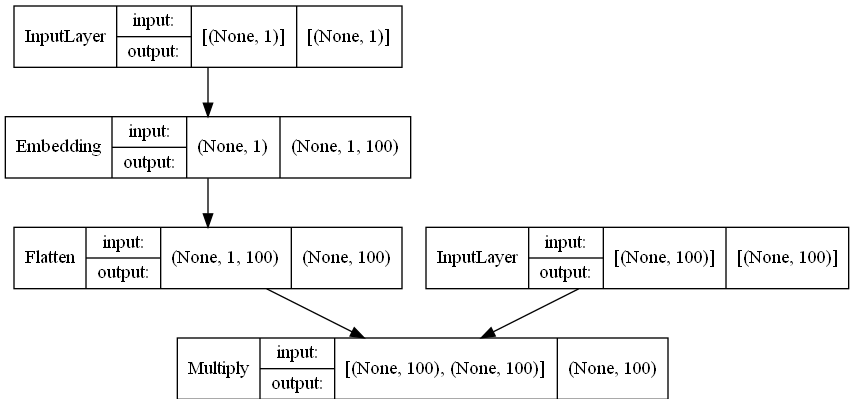
\includegraphics[height=0.3\textheight]{kapitel/5_ergebnisse/architectures/densegan_generator/input.png}
	\caption{Inputs des Dense-GAN-Generators}
	\label{architecture:densegan-gen-input}
\end{figure}

Auch der Generator besitzt drei aufeinanderfolgende Verabeitungsschichten (siehe \ref{architecture:densegan-gen-dense}).
Jedoch besteht diese Einheiten nicht nur aus einem DenseLayer und einer Aktivierungsfunktion.
Durch die Eingabe eines Zufallsvektors ist die Werteverteilung von Datensatz zu Datensatz sehr unterschiedlich.
Um das Training zu beschleunigen, wird zusätzlich eine BatchNormalization angewendet, welches die Werteverteilung angleichen sollte.

\begin{figure}[H]
	\centering
	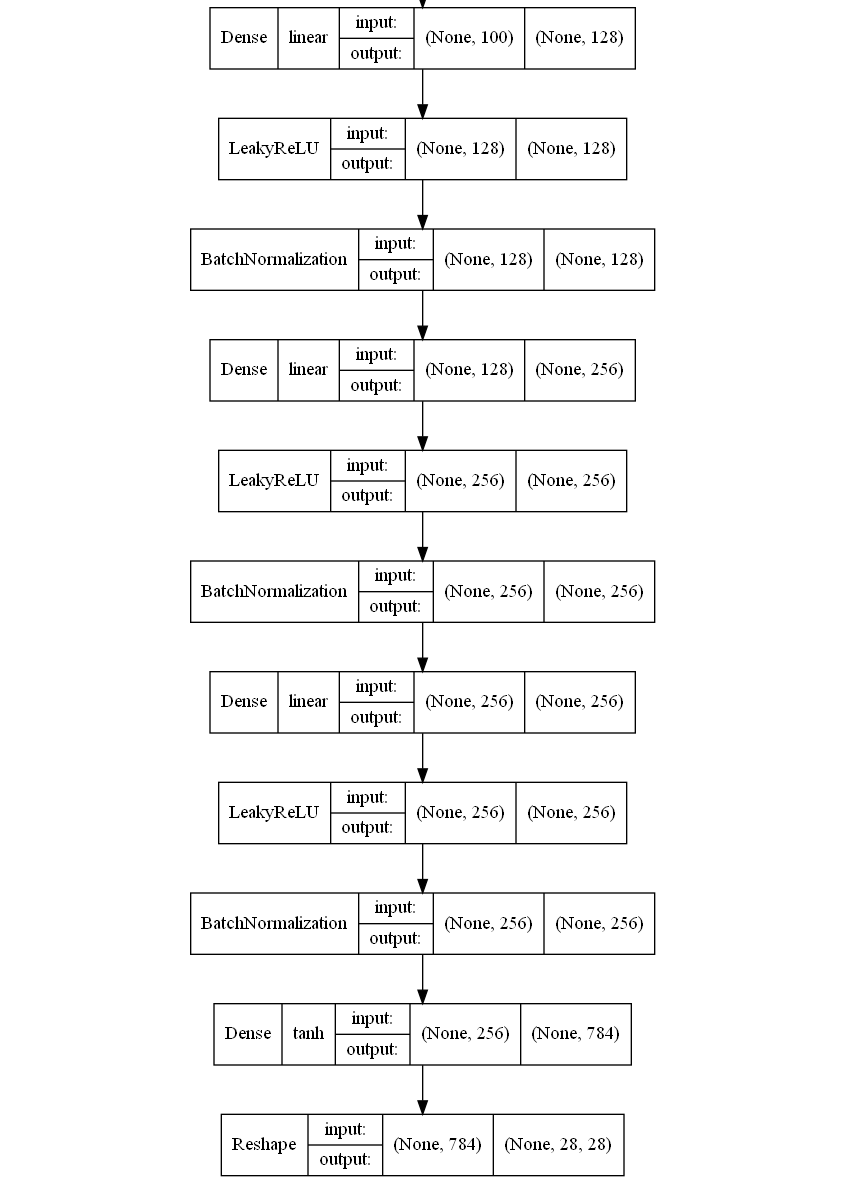
\includegraphics[width=0.6\textheight]{kapitel/5_ergebnisse/architectures/densegan_generator/output.png}
	\caption{Verabeitungs Schichten des Dense-GAN-Generators}
	\label{architecture:densegan-gen-dense}
\end{figure}

Um die Ausgabe des Generators zu erreichen, müssen nach den Verabeitungselementen eine letztes DenseLayer folgen, welches die Neuronen-Anzahl auf \textit{784} erhöht.
Anschließend werden diese in eine Matrix \textit{[28,28]} geformt, um ein generiertes Bild zu repräsentieren.
\newline

Sowohl die Architektur des Discriminators \cref{architecture:densegan-dis} als auch des Generators \cref{architecture:densegan-gen} ist in den Anlagen als volle Diagramme zu finden.

\subsection{DC-GAN}
\label{section:dc-gan-late-label}
Die Architektur dieses Modells basiert nicht auf anderen Papern oder Tutorials.
Der Hauptaspekt liegt hier in der Verwendung des Convolutional- und ConvolutionalTransposedLayer.
Diese sollen die in vorherigen Architektur verwendeten Dense-Schichten ersetzten.

\subsubsection{Discriminator}
Eine Besonderheit der Architektur liegt in der späten Fusionierung von Bild- und Labeldaten beim Discriminator.
Das bedeutet, dass die Bilddaten zunächst verarbeitet werden, bevor das Label einen Einfluss hat.
In der Abbildung \ref{architecture:dcgan-dis-bild} ist Verabeitung jenes Bild-Inputs visualisiert.
Wie man erkennen kann, existieren drei verschiedene Faltungsstufen, die jeweils aus einem ConvolutionalLayer, einer Aktivierungsfunktion und einem DropoutLayer bestehen.
\newline

Der Formfaktor bei ConvolutionalLayer unterscheidet sich deutlich zu denen des DenseLayer.
Wie man erkennen kann, wird hier mit dreidimensionalen Tensoren gearbeitet.
Dabei bewegt sich der Kernel über ersten beiden Achsen, wie im Kapitel 2.1.2 bereits beschrieben wurde.
Es wurden Kernel-Größe, Padding und Stride jeweils so gewählt, dass jeder Faltung die Bildgröße halbiert wird (bei der letzten Faltung wird auf \textit{4} aufgerundet).
Die letzte Dimension repräsentiert dabei verschiedene \textit{FeatureMaps}.
Das bedeutet, dass pro Eintrag in der dritten Dimension eine eigene Faltungsmatrix trainiert werden muss.
Beim ersten Verabeitungsschritt wird auf \textit{64} verschiedene \textit{FeatureMaps} aufgeteilt.
Anschließend wird die Anzahl verdoppelt, bis sie einen Wert von \textit{256} erreicht.

\begin{figure}[H]
	\centering
	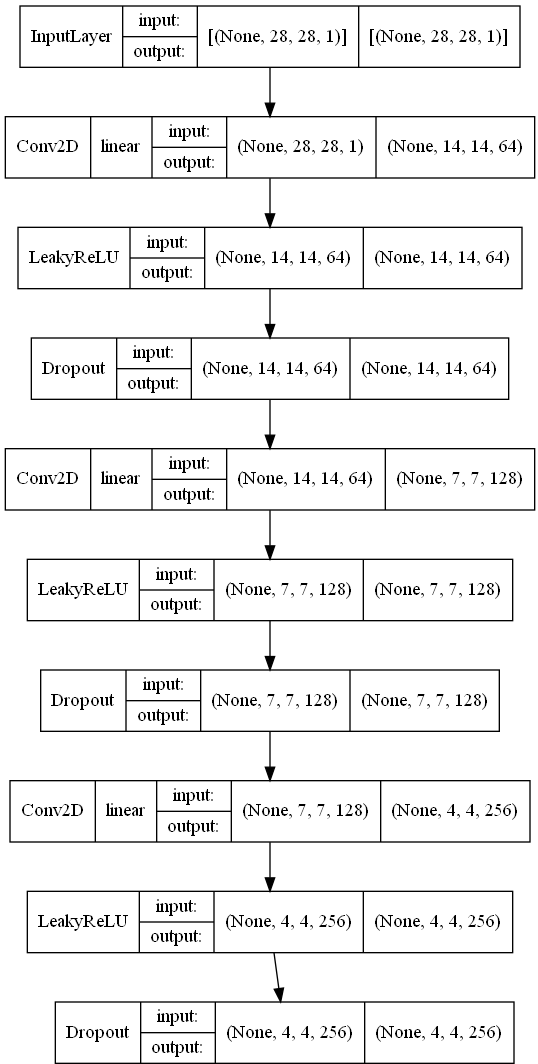
\includegraphics[width=0.45\textheight]{kapitel/5_ergebnisse/architectures/dcgan_disriminator/label_input.png}
	\caption{Bild-Input des DC-GAN-Discriminator}
	\label{architecture:dcgan-dis-bild}
\end{figure}

Die Bildinformationen haben dementsprechend nach der Verarbeitung einen Formfaktor von \textit{[4,4,256]}.
Damit sie mit dem Label multipliziert werden können, muss das Label die Größe \textit{[4,4,1]} annehmen.
Wie in der Abbildung \ref{architecture:dcgan-dis-label} aufgezeigt, wird das Labels über ein EmbeddingLayer in einen \textit{50} Neuronen langen Vektor transformiert.
Es wurde bereits beschrieben, dass dieses \textit{Embedden}, dem Zuweisen eines einzigartigen Identifikations-Vektor jeder Klasse dient.
Anschließend wird in einem DenseLayer die Neuronenanzahl auf \textit{16} komprimiert, um darauffolgend in die geforderte Form \textit{[4,4,1]} überführt zu werden.

\begin{figure}[H]
	\centering
	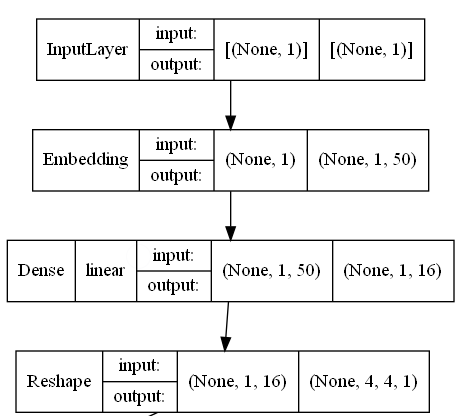
\includegraphics[height=0.3\textheight]{kapitel/5_ergebnisse/architectures/dcgan_disriminator/bild_input.png}
	\caption{Label-Input des DC-GAN-Discriminator}
	\label{architecture:dcgan-dis-label}
\end{figure}

Die Vereinigung selbst fällt wie gewohnt aus.
Nach der Multiplikation wird per FlattenLayer ein Vektor mit der Länge \textit{4096} erzeugt.
Anschließend wird er auf ein Neuron komprimiert und eine lineare Aktivierungsfunktion angewendet, wie in Abbildung \ref{architecture:dcgan-dis-output} zu erkennen ist.

\begin{figure}[H]
	\centering
	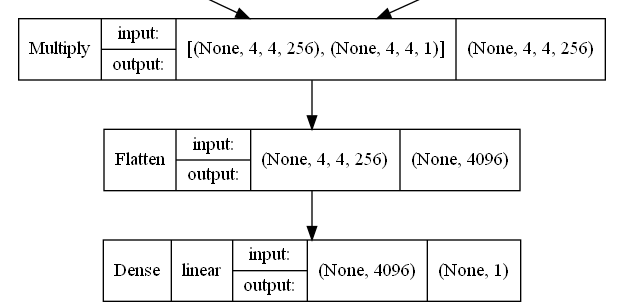
\includegraphics[height=0.2\textheight]{kapitel/5_ergebnisse/architectures/dcgan_disriminator/output.png}
	\caption{Output des DC-GAN-Discriminator}
	\label{architecture:dcgan-dis-output}
\end{figure}

\subsubsection{Generator}
Der Generator setzt zu Verarbeitung auf das ConvolutionalTransposedLayer.
Damit drei dieser Schichten implementiert werden können, muss das MultiplikationsLayer eine ähnlichen Output haben, wie der Diskriminator nach seinen Faltungsschichten.
Das kommt davon, dass das ConvolutionalTransposedLayer im Grunde nur ein umgekehrtes ConvolutionalLayer darstellt.
Dafür wurde sich für eine Formgröße \textit{[7,7,255]} entschieden.
Damit das Verhältnis zwischen Label und Bild / Latent identisch zum Discriminator ist, wird der Label-Skalar zu \textit{[7,7,1]} und der Zufallsvektor zu \textit{[7,7,255]} transformiert.
Das Verfahren dieser Transformation entspricht den bereits gezeigten Techniken und kann in der Abbildung \ref{architecture:dcgan-gen-intpu} betrachtet werden.

\begin{figure}[H]
	\centering
	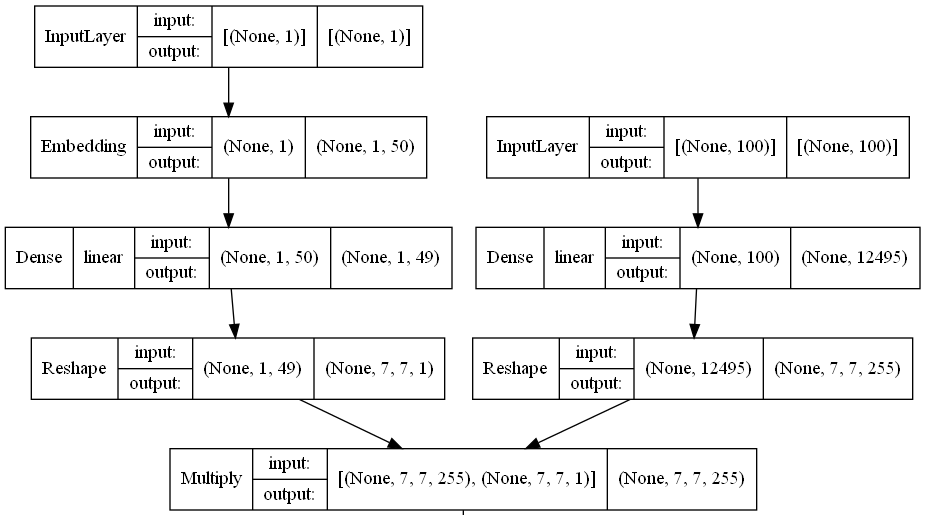
\includegraphics[height=0.3\textheight]{kapitel/5_ergebnisse/architectures/dcgan_generator/input.png}
	\caption{Inputs des DC-GAN-Generators}
	\label{architecture:dcgan-gen-intpu}
\end{figure}

Auch im DC-GAN Generator findet man drei Verarbeitungsabschnitte, wie in Abbildung \ref{architecture:dcgan-dis-output} visualisiert.
In den ersten beiden Schritten wird nach der Transpose-Schicht eine BatchNormalization und LeakyReLU-Aktivierung angewendet.
Auch hier wird die Normalisierung aufgrund des stark fluktuierenden Latend-Vektor angewendet.
Nach dem letzten ConvolutionalTransposedLayer, bei dem auch die gewünschte Größe von \textit{[28,28,1]} erreicht wird, nur noch eine Tanh-Aktivierungsfunktion ausgeführt.
Die letzte Schicht dient lediglich dazu, die 3. Achse zu entfernen.

\begin{figure}[H]
	\centering
	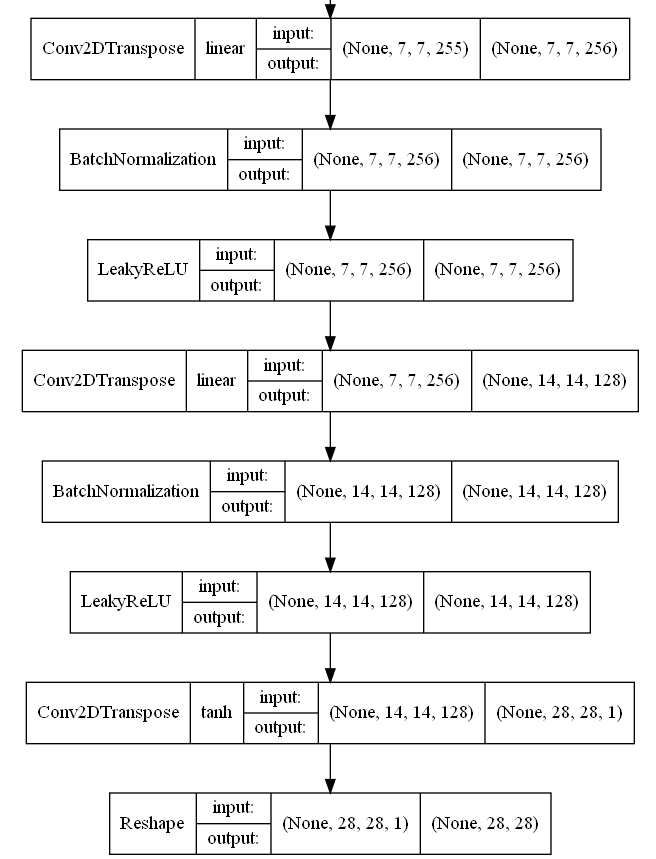
\includegraphics[width=0.6\textheight]{kapitel/5_ergebnisse/architectures/dcgan_generator/output.png}
	\caption{Verabeitungs Schichten des DC-GAN-Generators}
	\label{architecture:dcgan-gen-output}
\end{figure}

Ein Diagramm mit den vollen Architekturen befinden sich im Anhang (Discriminator \cref{architecture:dcgan-dis} und Generator \cref{architecture:dcgan-gen}).
